% Capitolul 0: Introducere
% Statistică pe Piețe Financiare
% Program de licență, Academia de Studii Economice din București

\documentclass[9pt, aspectratio=169, t]{beamer}

% Asigură încadrarea conținutului pe diapozitive
\setbeamersize{text margin left=8mm, text margin right=8mm}

%=============================================================================
% CONFIGURARE TEMĂ ȘI STIL
%=============================================================================
\usetheme{default}

% Color Palette
\definecolor{MainBlue}{RGB}{26, 58, 110}
\definecolor{AccentBlue}{RGB}{26, 58, 110}
\definecolor{IDAred}{RGB}{205, 0, 0}
\definecolor{DarkGray}{RGB}{51, 51, 51}
\definecolor{MediumGray}{RGB}{128, 128, 128}
\definecolor{LightGray}{RGB}{248, 248, 248}
\definecolor{VeryLightGray}{RGB}{235, 235, 235}
\definecolor{KeynoteGray}{RGB}{218, 218, 218}
\definecolor{SectionGray}{RGB}{120, 120, 120}
\definecolor{FooterGray}{RGB}{100, 100, 100}
\definecolor{Crimson}{RGB}{220, 53, 69}
\definecolor{Forest}{RGB}{46, 125, 50}
\definecolor{Amber}{RGB}{181, 133, 63}
\definecolor{Orange}{RGB}{230, 126, 34}
\definecolor{Purple}{RGB}{142, 68, 173}

% Gradient background
\setbeamertemplate{background}{%
    \begin{tikzpicture}[remember picture, overlay]
        \shade[shading=axis, shading angle=315,
        top color=white, bottom color=KeynoteGray]
        (current page.south west) rectangle (current page.north east);
    \end{tikzpicture}%
}
\setbeamercolor{background canvas}{bg=}

\setbeamercolor{palette primary}{bg=MainBlue, fg=white}
\setbeamercolor{palette secondary}{bg=MainBlue!85, fg=white}
\setbeamercolor{palette tertiary}{bg=MainBlue!70, fg=white}
\setbeamercolor{structure}{fg=MainBlue}
\setbeamercolor{title}{fg=IDAred}
\setbeamercolor{frametitle}{fg=IDAred, bg=}
\setbeamercolor{block title}{bg=MainBlue, fg=white}
\setbeamercolor{block body}{bg=VeryLightGray, fg=DarkGray}
\setbeamercolor{block title alerted}{bg=Crimson, fg=white}
\setbeamercolor{block body alerted}{bg=Crimson!8, fg=DarkGray}
\setbeamercolor{block title example}{bg=Forest, fg=white}
\setbeamercolor{block body example}{bg=Forest!8, fg=DarkGray}
\setbeamercolor{item}{fg=MainBlue}

% Culori subsol
\setbeamercolor{author in head/foot}{fg=FooterGray, bg=}
\setbeamercolor{title in head/foot}{fg=FooterGray, bg=}
\setbeamercolor{date in head/foot}{fg=FooterGray, bg=}
\setbeamercolor{section in head/foot}{fg=FooterGray, bg=}
\setbeamercolor{subsection in head/foot}{fg=FooterGray, bg=}

% Stiluri marcatori
\setbeamertemplate{itemize item}{\color{MainBlue}$\boxdot$}
\setbeamertemplate{itemize subitem}{\color{MainBlue}$\blacktriangleright$}
\setbeamertemplate{itemize subsubitem}{\color{MainBlue}\tiny$\bullet$}
\setbeamertemplate{itemize/enumerate body begin}{\normalsize}
\setbeamertemplate{itemize/enumerate subbody begin}{\normalsize}

% Spațiere elemente
\setlength{\leftmargini}{10pt}
\setlength{\leftmarginii}{10pt}
\makeatletter
\def\@listi{\leftmargin\leftmargini \topsep 0pt \parsep 0pt \itemsep 0pt}
\def\@listii{\leftmargin\leftmarginii \topsep 0pt \parsep 0pt \itemsep 0pt}
\makeatother

\setbeamertemplate{navigation symbols}{}

%=============================================================================
% ANTET PERSONALIZAT
%=============================================================================
\setbeamertemplate{headline}{%
    \vskip10pt%
    \hbox to \paperwidth{%
        \hskip0.5cm%
        {\small\color{FooterGray}\renewcommand{\hyperlink}[2]{##2}\insertsectionhead}%
        \hfill%
        \textcolor{FooterGray}{\small\insertframenumber}%
        \hskip0.5cm%
    }%
    \vskip4pt%
    {\color{FooterGray}\hrule height 0.4pt}%
}

%=============================================================================
% SUBSOL PERSONALIZAT
%=============================================================================
\usepackage{fontawesome5}

\setbeamertemplate{footline}{%
    {\color{FooterGray}\hrule height 0.4pt}%
    \vskip4pt%
    \hbox to \paperwidth{%
        \hskip0.5cm%
        \textcolor{FooterGray}{\small Statistică pe Piețe Financiare}%
        \hfill%
        \raisebox{-0.1em}{%
            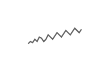
\begin{tikzpicture}[x=0.08em, y=0.08em, line width=0.4pt]
                \draw[FooterGray] (0,3) -- (1,4) -- (2,3.5) -- (3,5) -- (4,4) -- (5,6) -- (6,5.5) -- (7,4) -- (8,5) -- (9,7) -- (10,6) -- (11,5) -- (12,6.5) -- (13,8) -- (14,7) -- (15,6) -- (16,7.5) -- (17,9) -- (18,8) -- (19,7) -- (20,8.5) -- (21,10) -- (22,9) -- (23,8) -- (24,9.5);
            \end{tikzpicture}%
        }%
        \hskip0.5cm%
    }%
    \vskip6pt%
}

%=============================================================================
% PACHETE
%=============================================================================
\usepackage[utf8]{inputenc}
\usepackage[T1]{fontenc}
\usepackage{amsmath, amssymb, amsthm}
\usepackage{mathtools}
\usepackage{bm}
\usepackage{tikz}
\usetikzlibrary{arrows.meta, positioning, shapes, calc, decorations.pathreplacing, shadings}
\usepackage{booktabs}
\usepackage{multirow}
\usepackage{array}
\usepackage{graphicx}
\usepackage{hyperref}
\usepackage{colortbl}
\usepackage{listings}
\lstset{language=Python, basicstyle=\ttfamily\scriptsize, keywordstyle=\color{MainBlue}\bfseries,
  commentstyle=\color{Forest}, stringstyle=\color{Crimson}, breaklines=true,
  frame=none, backgroundcolor=\color{VeryLightGray}, xleftmargin=2mm}
\hypersetup{colorlinks=true, linkcolor=MainBlue, urlcolor=MainBlue}
\graphicspath{{../../logos/}{../../charts/}{../../photos/}}
\hfuzz=2pt
\vfuzz=2pt

%=============================================================================
% COMANDA QUANTLET
%=============================================================================
\newcommand{\quantlet}[2]{%
    \hfill\href{#2}{%
        \raisebox{-0.15em}{
\includegraphics[height=0.7em]{ql_logo.png}}%
        \textcolor{MainBlue}{\tiny\ #1}%
    }%
}

%=============================================================================
% PAGINĂ TITLU PERSONALIZATĂ
%=============================================================================
\defbeamertemplate*{title page}{hybrid}[1][]
{
    \vspace{0.2cm}
    \begin{center}
        \href{https://www.ase.ro}{
\includegraphics[height=1.0cm]{ase_logo.png}}\hspace{0.3cm}%
        \href{https://theida.net}{
\includegraphics[height=1.0cm]{ida_logo.png}}\hspace{0.3cm}%
        \href{https://blockchain-research-center.com}{
\includegraphics[height=1.0cm]{brc_logo.png}}\hspace{0.3cm}%
        \href{https://www.ai4efin.ase.ro}{
\includegraphics[height=1.0cm]{ai4efin_logo.png}}\hspace{0.3cm}%
        \href{https://ipe.ro/new}{
\includegraphics[height=1.0cm]{acad_logo.png}}\hspace{0.3cm}%
        \href{https://www.digital-finance-msca.com}{
\includegraphics[height=1.0cm]{msca_logo.png}}%
    \end{center}

    \vspace{0.6cm}

    \begin{center}
        \begin{minipage}{0.1\textwidth}
            \centering
            \href{https://quantlet.com}{
\includegraphics[height=1.1cm]{ql_logo.png}}
        \end{minipage}%
        \begin{minipage}{0.78\textwidth}
            \centering
            {\LARGE\bfseries\usebeamercolor[fg]{title}\inserttitle}

            \vspace{0.3cm}

            {\usebeamerfont{subtitle}\usebeamercolor[fg]{title}\insertsubtitle}
        \end{minipage}%
        \begin{minipage}{0.1\textwidth}
            \centering
            \href{https://quantinar.com}{
\includegraphics[height=1.1cm]{qr_logo.png}}
        \end{minipage}
    \end{center}

    \vspace{0.6cm}

    \hspace{0.5cm}{\usebeamerfont{author}\insertauthor}

    \vspace{0.3cm}

    \hspace{0.5cm}\begin{minipage}[t]{0.9\textwidth}
        \raggedright\small\insertinstitute
    \end{minipage}
}

%=============================================================================
% MEDII PENTRU TEOREME
%=============================================================================
\theoremstyle{definition}
\setbeamertemplate{theorems}[numbered]
\newtheorem{defn}{Definiție}
\newtheorem{thm}{Teoremă}
\newtheorem{prop}{Propoziție}
\newtheorem{rmk}{Observație}

%=============================================================================
% CENTRED MINIPAGE
%=============================================================================
\newenvironment{cminipage}[1]{%
    \par\noindent\hfill\begin{minipage}{#1}\ignorespaces
}{%
    \end{minipage}\hfill\null\par
}

%=============================================================================
% COMENZI PERSONALIZATE
%=============================================================================
\newcommand{\E}{\mathbb{E}}
\newcommand{\Var}{\text{Var}}
\newcommand{\Cov}{\text{Cov}}
\newcommand{\Corr}{\text{Corr}}
\newcommand{\R}{\mathbb{R}}
\newcommand{\N}{\mathbb{N}}
\newcommand{\Z}{\mathbb{Z}}
\newcommand{\B}{\mathbf{B}}
\newcommand{\imark}{\textcolor{MainBlue}{\textbullet}}

%=============================================================================
% INFORMAȚII TITLU
%=============================================================================
\title[Statistică pe Piețe Financiare]{Statistică pe Piețe Financiare}
\subtitle{Introducere}
\author[D.T. Pele, A. Amza]{Daniel Traian PELE \\ Antoaneta Amza}
\institute{Academia de Studii Economice din București\\
IDA Institute Digital Assets\\
Blockchain Research Center\\
AI4EFin Artificial Intelligence for Energy Finance\\
Academia Română, Institutul de Prognoză Economică\\
MSCA Digital Finance}
\date{}

\begin{document}

% Pagina de titlu (fără antet/subsol)
{
\setbeamertemplate{headline}{}
\setbeamertemplate{footline}{}
\begin{frame}
    \titlepage
\end{frame}
}

%=============================================================================
% MOTIVAȚIE
%=============================================================================
\section{Motivație}

\begin{frame}{Este piața financiară!}
\begin{center}
    \vspace{0.5cm}
    {\large\textit{``It's the economy, Stupid!''}}

    \vspace{0.3cm}

    {\small --- James Carville, 1992 (strategul campaniei lui Bill Clinton)}

    \vspace{1cm}

    {\Large\textbf{\textcolor{IDAred}{Este piața financiară!}}}

    \vspace{0.5cm}

    {\small Piețele financiare sunt coloana vertebrală a economiei moderne.\\
    Înțelegerea proprietăților lor statistice este esențială pentru luarea deciziilor informate.}
\end{center}
\end{frame}

\begin{frame}{De ce studiem Statistica pe Piețe Financiare (SFM)?}
\begin{itemize}
    \item Piețele financiare sunt extrem de complexe, dinamice și volatile.
    \item Compromisurile între risc și randament trebuie analizate cu atenție pentru a lua decizii investiționale informate.
    \item Evaluarea prețurilor, acoperirea riscului și managementul portofoliului depind de modele cantitative și statistice.
    \item Luarea deciziilor bazate pe date este fundamentală în finanțe, mai ales odată cu apariția big data și a învățării automate.
    \item Finanțele moderne se bazează puternic pe tehnici statistice pentru
    \begin{itemize}
        \item Modele de evaluare a activelor (CAPM, APT)
        \item Managementul riscului (VaR, Expected Shortfall)
        \item Optimizarea portofoliului (Analiza Medie-Varianță, Black-Litterman)
        \item Tranzacționare algoritmică și analiza microstructurii pieței
    \end{itemize}
\end{itemize}
\end{frame}

\begin{frame}{Aplicații practice ale SFM}
\begin{itemize}
    \item Evaluarea activelor și predicția randamentelor
    \begin{itemize}
        \item Determinarea prețului corect al activelor financiare folosind modele statistice.
        \item Capital Asset Pricing Model (CAPM), modele multifactoriale Fama-French.
        \item Modele de predicție a randamentelor bazate pe învățare automată.
        \item Arbitraj statistic și investiții bazate pe factori.
    \end{itemize}
    \item Managementul riscului și stabilitatea financiară
    \begin{itemize}
        \item Cuantificarea riscului financiar, măsurarea volatilității și gestionarea riscului de portofoliu.
        \item Value at Risk (VaR) și Conditional Value at Risk (CVaR).
        \item Evaluarea în măsură neutră la risc și simulări Monte Carlo.
        \item Teoria Valorilor Extreme (EVT) pentru estimarea riscului de coadă.
        \item Teste de stres și analiză de scenarii pentru conformitatea reglementară (Basel III, Solvency II).
    \end{itemize}
\end{itemize}
\end{frame}

\begin{frame}{Aplicații practice ale SFM}
\begin{itemize}
    \item Tranzacționare algoritmică și de înaltă frecvență
    \begin{itemize}
        \item Obiectiv: Utilizarea modelelor cantitative pentru dezvoltarea strategiilor de tranzacționare profitabile.
        \item Arbitraj statistic folosind modele de co-integrare.
        \item Modelarea impactului pe piață și strategii de execuție.
        \item Modele de market-making și furnizare de lichiditate.
        \item Tranzacționare de înaltă frecvență folosind învățare automată (LSTM-uri, deep reinforcement learning).
    \end{itemize}
    \item Riscul de credit și stabilitatea financiară
    \begin{itemize}
        \item Obiectiv: Evaluarea probabilității de nerambursare și a stabilității sistemului financiar.
        \item Modele de scoring de credit (ex. Regresie Logistică, Random Forests).
        \item Modele structurale ale riscului de credit (Modelul Merton).
        \item Modele de formă redusă (modelul Jarrow-Turnbull).
        \item Indicatori de risc sistemic și modelarea contagiunii.
    \end{itemize}
\end{itemize}
\end{frame}

\begin{frame}{Cum ajută statistica pe piețele financiare}
\begin{itemize}
    \item Detectarea tendințelor și anomaliilor de piață
    \begin{itemize}
        \item Identificarea oportunităților de arbitraj, a tiparelor de revenire la medie și a tendințelor sezoniere.
    \end{itemize}
    \item Construirea modelelor predictive pentru prețurile activelor
    \begin{itemize}
        \item Aplicarea învățării automate, a analizei seriilor de timp și a metodelor econometrice.
    \end{itemize}
    \item Măsurarea și gestionarea riscului financiar
    \begin{itemize}
        \item Utilizarea indicatorilor statistici de risc, a testelor de stres și a analizei de scenarii.
    \end{itemize}
    \item Validarea teoriilor financiare cu date empirice
    \begin{itemize}
        \item Ipoteza Piețelor Eficiente (EMH)
        \item Teorii din Finanțele Comportamentale
        \item Modele de evaluare a activelor
    \end{itemize}
\end{itemize}
\end{frame}

\begin{frame}{Ascensiunea mașinilor}
\begin{columns}[T]
\begin{column}{0.48\textwidth}
\begin{itemize}
    \item \underline{Cray 2}: cel mai rapid supercomputer din lume: 1985--1990
    \item 1.9 GFLOPs
    \item 5,500 livre
    \item \$49,863,243.49 milioane (dolari actuali)
    \item $10^{\wedge}$(G=9, T=12, P=15, E=18)
\end{itemize}

\vspace{0.5cm}

{\small\textcolor{IDAred}{G = Giga, T = Tera, P = Peta, E = Exa}}
\end{column}
\begin{column}{0.48\textwidth}
\begin{center}
    {\small\textit{[Imagine supercomputer Cray 2]}}
\end{center}
\end{column}
\end{columns}
\end{frame}

\begin{frame}{Ascensiunea mașinilor}
\begin{columns}[T]
\begin{column}{0.48\textwidth}
\begin{itemize}
    \item 2016 iPhone 7, 178 GFLOPs
    \item 2021 iPhone 13, 1200 GFLOPs
    \item 2025 iPhone 16, 2.15 TFLOPS
    \item 170 g = 1K EUR
    \item $10^{\wedge}$(G9, T12, P15, E18)
\end{itemize}
\end{column}
\begin{column}{0.48\textwidth}
\begin{center}
    {\small\textit{[Imagini cu cipul A18, placa Cray-2 și iPhone]}}
\end{center}
\end{column}
\end{columns}
\end{frame}

\begin{frame}{Repere ale criptomonedelor}
\begin{center}
    {\small\textit{[Graficul indicelui S\&P Cryptocurrency MegaCap, 2017--2025]}}

    \vspace{0.3cm}

    Evenimente cheie adnotate pe grafic:
\end{center}
\begin{itemize}
    \item 2017 Boom și 2018 Prăbușirea bulei
    \item 2020 Mai: A 3-a înjumătățire Bitcoin
    \item 2020 Boom și 2021 Prăbușirea bulei
    \item 2021 Boom NFT
    \item 2022 Apr: Reglementare SEC
    \item 2022 Nov: Falimentul FTX
    \item 2024 Ian: BTC Spot ETF
    \item 2024 Apr: A 4-a înjumătățire BTC
    \item 2024 Mai: ETH Spot ETF
    \item 2024 Nov: Trump ales
\end{itemize}
{\small\textit{Sursa datelor: S\&P Cryptocurrency MegaCap Index -- 14 ian. 2025}}
\end{frame}

\begin{frame}{Bule speculative}
\begin{columns}[T]
\begin{column}{0.55\textwidth}
{\small
În primăvara anului 1720, Sir Isaac Newton deținea acțiuni la South Sea Company, cea mai căutată acțiune din Anglia. Pe măsură ce a apărut un zvon printre oameni că s-a descoperit minereu de argint/aur, aceasta era o ``știre falsă'' așa cum le numim astăzi. Marele fizician a mormăit că `\textcolor{IDAred}{putea calcula mișcările corpurilor cerești, dar nu nebunia oamenilor}.' Newton și-a vândut acțiunile South Sea, obținând un profit de 100\% totalizând \pounds 7,000. Dar la doar câteva luni, prins de entuziasmul sălbatic al pieței, Newton a cumpărat din nou la un preț mult mai mare --- și a pierdut \pounds 20,000 (sau mai mult de \pounds 5 milioane în banii din 2025). Pentru tot restul vieții, a interzis oricui să rostească cuvintele `South Sea' în prezența sa.
}

\vspace{0.2cm}

{\small\textit{[Graficul acțiunilor South Sea, decembrie 1718 -- decembrie 1721]}}
\end{column}
\begin{column}{0.42\textwidth}
\begin{center}
    {\small\textit{[Portretul lui Newton]}}

    \vspace{0.3cm}

    {\small\textit{[Ilustrație cu mărul lui Newton]}}

    \vspace{0.2cm}

    {\small \href{https://www.ams.org/journals/notices/201906/rnoti-p952.pdf}{\underline{Andrew Odlyzko (2019)}}}
\end{center}
\end{column}
\end{columns}
\end{frame}

\begin{frame}{Valori intrinseci ale CC}
\begin{columns}[T]
\begin{column}{0.45\textwidth}
\begin{itemize}
    \item În cele din urmă zero sau adoptare în continuare?
    \item Legea lui Metcalfe: $p$ capitalizare de piață,
    \begin{itemize}
        \item $p = e^{\alpha_0} u^{\beta_0}$ și $\beta_0 = 2$.
        \item $u$: \# utilizatori activi, adică adrese
    \end{itemize}
    \item Legea (generalizată) a lui Metcalfe:
    \[
    \log(p) = \alpha + \beta \log(u) + \varepsilon
    \]
\end{itemize}

\vspace{0.5cm}

{\small \href{https://doi.org/10.1016/j.econlet.2018.09.007}{\underline{Wheatley S et al (2018)}}}
\end{column}
\begin{column}{0.52\textwidth}
\begin{center}
    {\small\textit{[Grafic log-log Capitalizare de piață (USD) vs Utilizatori activi, 2010--2025]}}

    \vspace{1cm}

    \quantlet{CC returns}{https://github.com/QuantLet}
\end{center}
\end{column}
\end{columns}
\end{frame}

\begin{frame}{Bule}
\begin{columns}[T]
\begin{column}{0.42\textwidth}
\begin{itemize}
    \item Raportul Piață-Metcalfe
    \[
    \text{MMV}_i = \frac{p_i}{e^{\alpha} u_i^{\beta}}
    \]
    după ajustarea regresiei log-log,
    \[
    (\alpha, \beta) = (-1.75, 2.12)
    \]
    \item Șase bule identificate
\end{itemize}

\vspace{0.5cm}

{\small \href{https://doi.org/10.1016/j.econlet.2018.09.007}{\underline{Wheatley S et al (2018)}}}
\end{column}
\begin{column}{0.55\textwidth}
\begin{center}
    {\small\textit{[Grafic raport MMV, 2010--2024, perioade de bule colorate]}}

    \vspace{1cm}

    \quantlet{CC returns}{https://github.com/QuantLet}
\end{center}
\end{column}
\end{columns}
\end{frame}

\begin{frame}{Noul Aur}
\begin{columns}[T]
\begin{column}{0.55\textwidth}
\begin{itemize}
    \item Capitalizare de piață Aur (27 apr. 2023) 13,192 Miliarde USD
    \item Capitalizare de piață BTC (27 apr. 2023) \quad 559 Miliarde USD
\end{itemize}

\hfill{\small 4.2\%}

\vspace{0.3cm}

\begin{itemize}
    \item Capitalizare de piață Aur (16 ian. 2025) 18.318 Trilioane USD
    \item Capitalizare de piață BTC (16 ian. 2025) \quad 1.972 Trilioane USD
\end{itemize}

\hfill{\small 9.29\%}

\vspace{0.3cm}

Dacă BTC și CC sunt văzute ca rezervă de valoare, atunci prețul poate crește încă mult.

\vspace{0.2cm}

{\small \href{https://companiesmarketcap.com/bitcoin/marketcap/}{\underline{Istoricul capitalizării de piață a Bitcoin}}}
\end{column}
\begin{column}{0.42\textwidth}
\begin{center}
    {\small\textit{[Imagine monedă de aur + logo Bitcoin]}}
\end{center}
\end{column}
\end{columns}
\end{frame}

\begin{frame}{Modelul de volatilitate stocastică cu salturi corelate}
\begin{columns}[T]
\begin{column}{0.55\textwidth}
\[
\frac{dS_t}{S_t} = r\,dt + \sqrt{V_t}\,dW_t^s + Z_t^y\,dN_t,
\]
\[
dV_t = \kappa(\theta - V_t)\,dt + \sigma_v\sqrt{V_t}\,dW_t^v + Z_t^v\,dN_t,
\]
\[
\Cov(dW_t^s, dW_t^v) = \rho\,dt, \quad P(dN_t = 1) = \lambda\,dt
\]
\[
Z_t^v \sim \text{Exp}(\mu_v), \quad Z_t^y | Z_t^v \sim N(\mu_y + \rho_j Z_t^v, \sigma_y^2).
\]

\vspace{0.3cm}

{\small\textit{[Boxplot-uri și serii de timp RMSE in-sample și out-of-sample pentru modelele BS, SV, SVJ, SVCJ]}}
\end{column}
\begin{column}{0.42\textwidth}
{\small
\begin{tabular}{lcccc}
\toprule
 & BS & SV & SVJ & SVCJ \\
\midrule
$\sigma$ & 0.0278 & & & \\
$\rho$ & & 0.1462 & $-0.3310$ & $-0.6245$ \\
$\kappa$ & & 0.2203 & 1.5459 & 0.7425 \\
$\theta$ & & 0.0006 & 0.0008 & 0.0008 \\
$V_0$ & & 0.0013 & 0.0009 & 0.0009 \\
$\sigma_v$ & & 0.0216 & 0.0368 & 0.0489 \\
$\lambda$ & & & 0.0040 & 0.0033 \\
$\mu_v$ & & & 0.2359 & 0.3166 \\
$\rho_j$ & & & & $-1.0821$ \\
$\sigma_y$ & & & 0.1890 & 0.1267 \\
$\mu_v$ & & & & 0.0206 \\
\bottomrule
\end{tabular}
}

\vspace{0.2cm}

{\scriptsize \href{https://doi.org/10.1016/j.frl.2021.102483}{\underline{Teng \& Haerdle (2022)}} Financial analytics of inverse BTC options in a stoch.\ vol.\ world}
\end{column}
\end{columns}
\end{frame}

%=============================================================================
% CUPRINS
%=============================================================================
{
\setbeamertemplate{headline}{%
    \vskip10pt%
    \hbox to \paperwidth{%
        \hskip0.5cm%
        \hfill%
        \hskip0.5cm%
    }%
    \vskip4pt%
    {\color{FooterGray}\hrule height 0.4pt}%
}
\begin{frame}{}
    {\color{FooterGray}\hrule height 0.4pt}

    \vspace{0.3cm}

    {\Large\textcolor{IDAred}{\textbf{Cuprins}}}

    \vspace{0.4cm}

    \begin{enumerate}
        \item Motivație \checkmark
        \item Prezentare generală a cursului
        \item Resurse
        \item Notare
        \item Bibliografie
    \end{enumerate}
\end{frame}
}

%=============================================================================
% PREZENTARE GENERALĂ A CURSULUI
%=============================================================================
\section{Prezentare generală a cursului}

\begin{frame}{Obiectivele cursului}
\begin{itemize}
    \item Înțelegerea metodelor statistice fundamentale aplicate în finanțe.
    \item Dezvoltarea expertizei în teoria probabilităților și aplicațiile acesteia pe piețele financiare.
    \item Învățarea modelelor de serii de timp (ARIMA, GARCH) pentru analiza datelor financiare.
    \item Studierea Ipotezei Piețelor Eficiente (EMH) și a validării sale empirice.
    \item Explorarea Ipotezei Piețelor Fractale (FMH) și a proceselor cu memorie lungă.
    \item Înțelegerea grupării volatilității și a implicațiilor acesteia pentru modelarea riscului.
    \item Analiza indicatorilor de risc precum VaR, CVaR și măsurile de risc sistemic.
    \item Învățarea modelelor de risc de credit și a rolului lor în stabilitatea financiară.
    \item Lucrul cu seturi de date financiare reale și implementarea în Python/R.
\end{itemize}
\end{frame}

\begin{frame}{Teme principale abordate}
\begin{itemize}
    \item Probabilități și metode statistice în finanțe
    \begin{itemize}
        \item Distribuțiile de probabilitate ale randamentelor activelor (Normală, Log-normală, t-distribuție, Distribuții stabile).
        \item Simulări Monte Carlo pentru evaluare și estimarea riscului.
        \item Procese stocastice în finanțe (mișcarea Browniană, procese L\'{e}vy, Mișcarea Browniană Fracțională).
    \end{itemize}
    \item Analiza seriilor de timp și prognoză
    \begin{itemize}
        \item Modele autoregresive (AR, ARMA, ARIMA) pentru predicția randamentelor.
        \item Modelarea volatilității: GARCH, EGARCH, TGARCH.
        \item Gruparea volatilității: De ce volatilitatea este persistentă și grupată pe piețele financiare.
    \end{itemize}
    \item Ipoteza Piețelor Eficiente (EMH) și Ipoteza Piețelor Fractale (FMH)
    \begin{itemize}
        \item EMH: Eficiența de formă slabă, semi-puternică și puternică.
        \item Teste empirice ale EMH folosind tehnici statistice (mers aleatoriu, autocorelație, teste de raport al varianței).
        \item FMH: Comportamentul nestaționar al piețelor financiare, auto-similaritate și procese cu memorie lungă.
    \end{itemize}
\end{itemize}
\end{frame}

\begin{frame}{Teme principale abordate}
\begin{itemize}
    \item Gruparea volatilității și stabilitatea financiară
    \begin{itemize}
        \item Gruparea volatilității: De ce piețele financiare prezintă perioade persistente de volatilitate ridicată/scăzută.
        \item Efectul de levier: Cum șocurile negative cresc volatilitatea mai mult decât șocurile pozitive.
        \item Indicatori de risc: Value at Risk (VaR), Conditional VaR (CVaR).
    \end{itemize}
    \item Riscul de credit și predicția nerambursării
    \begin{itemize}
        \item Modele de scoring de credit
        \item Teste de stres și cadrul reglementar Basel III.
    \end{itemize}
\end{itemize}
\end{frame}

%=============================================================================
% RESURSE
%=============================================================================
\section{Resurse}

\begin{frame}{Resurse}
\begin{itemize}
    \item \textbf{Manual principal}:
    \begin{itemize}
        \item H\"{a}rdle, W.K., Hautsch, N., Overbeck, L. (2017). \textit{Applied Quantitative Finance}. Springer.
    \end{itemize}
    \item \textbf{Lectură suplimentară}:
    \begin{itemize}
        \item Franke, J., H\"{a}rdle, W.K., Hafner, C.M. (2019). \textit{Statistics of Financial Markets: An Introduction}. 4th Edition, Springer.
        \item Tsay, R.S. (2010). \textit{Analysis of Financial Time Series}. 3rd Edition, Wiley.
        \item Campbell, J.Y., Lo, A.W., MacKinlay, A.C. (1997). \textit{The Econometrics of Financial Markets}. Princeton University Press.
    \end{itemize}
    \item \textbf{Software}: Python (statsmodels, scipy, arch), R
    \item \textbf{Resurse online}: Quantlet.com, depozite GitHub
\end{itemize}
\end{frame}

%=============================================================================
% NOTARE
%=============================================================================
\section{Notare}

\begin{frame}{Notare}
\begin{itemize}
    \item \textbf{Examen final}: 60\%
    \item \textbf{Proiect/Temă}: 40\%
    \begin{itemize}
        \item Proiecte individuale sau de grup folosind date financiare reale
        \item Implementare în Python sau R
        \item Raport scris + prezentare
    \end{itemize}
\end{itemize}
\end{frame}

%=============================================================================
% BIBLIOGRAFIE
%=============================================================================
\section{Bibliografie}

\begin{frame}{Bibliografie}
{\small
\begin{thebibliography}{99}
\bibitem{franke2019} Franke, J., H\"{a}rdle, W.K., Hafner, C.M. (2019). \textit{Statistics of Financial Markets: An Introduction}. 4th Edition, Springer.
\bibitem{tsay2010} Tsay, R.S. (2010). \textit{Analysis of Financial Time Series}. 3rd Edition, Wiley.
\bibitem{campbell1997} Campbell, J.Y., Lo, A.W., MacKinlay, A.C. (1997). \textit{The Econometrics of Financial Markets}. Princeton University Press.
\bibitem{hardle2017} H\"{a}rdle, W.K., Hautsch, N., Overbeck, L. (2017). \textit{Applied Quantitative Finance}. Springer.
\bibitem{wheatley2018} Wheatley, S., Sornette, D., Huber, T., Reppen, M., Gantner, R.N. (2018). Are Bitcoin Bubbles Predictable? \textit{Economics Letters}, 172, 149--152.
\bibitem{odlyzko2019} Odlyzko, A. (2019). Newton's Financial Misadventures in the South Sea Bubble. \textit{Notices of the AMS}, 66(7), 952--960.
\bibitem{teng2022} Teng, H., Haerdle, W.K. (2022). Financial analytics of inverse BTC options in a stochastic volatility world. \textit{Finance Research Letters}, 47, 102483.
\end{thebibliography}
}
\end{frame}

\end{document}
